% PROTON+ method figure, variant A: compact callout zoom into the DR queue.
% Real data: make_data.py (PW=3.60, PH=1.48) -> data.tex (FLAIR embeddings, ultra-widefield stream, seed 0, image t=413).
% Compile: tectonic -X compile --keep-logs fig_method.tex
\documentclass[tikz,border=1.5pt]{standalone}
\usepackage[T1]{fontenc}
\usepackage[scaled=0.92]{helvet}
\usepackage{amsmath,amssymb,pifont}
\usepackage{sansmath}
\usetikzlibrary{arrows.meta,calc,positioning,shadows.blur,backgrounds}
\renewcommand{\familydefault}{\sfdefault}
\makeatletter\renewcommand{\defaultscriptratio}{.8}\makeatother% larger sub/superscripts for print
\definecolor{acc}{HTML}{D55E00}\definecolor{accsoft}{HTML}{FDF0E6}\definecolor{acctint}{HTML}{FFF8F2}
\definecolor{cN}{HTML}{3B7DD8}\definecolor{cD}{HTML}{2E9E5B}\definecolor{cU}{HTML}{D64545}
\definecolor{ink}{HTML}{1F2328}\definecolor{mute}{HTML}{6B7280}\definecolor{line}{HTML}{9AA1AB}\definecolor{panel}{HTML}{F7F8FA}
\definecolor{zbg}{HTML}{F1F2F5}\colorlet{zline}{ink!50}
\def\bgNormal{0.528/0.117,0.571/0.065,1.479/0.353,0.620/0.260,0.727/0.049,0.916/0.124,1.040/0.134,0.728/0.045,0.769/0.056,0.865/0.057,0.746/0.203,0.502/0.061,0.812/0.100,1.781/0.159,1.058/0.195,0.364/0.063,0.779/0.072,1.555/0.086,1.160/0.282,0.563/0.093,0.568/0.071,1.040/0.216,1.217/0.166,0.508/0.077,0.350/0.167,1.069/0.041,0.862/0.070,0.575/0.107,1.060/0.111,1.026/0.052,1.005/0.111,1.140/0.171,0.643/0.200,0.749/0.156,0.738/0.147,1.412/0.116,1.642/0.140,1.493/0.281,0.511/0.103,1.581/0.064,0.538/0.196,0.648/0.321,0.906/0.154,0.718/0.269,1.257/0.063,0.482/0.095,0.644/0.068,0.348/0.082,0.649/0.168,0.797/0.126,0.999/0.085,1.927/0.079,0.320/0.158,0.393/0.067,0.270/0.191,0.508/0.209,0.428/0.072,0.391/0.176,0.405/0.104,0.183/0.246,0.201/0.238,0.193/0.203,0.524/0.160,0.183/0.173,0.232/0.079,0.176/0.186,0.162/0.249,0.426/0.126,0.167/0.212,0.162/0.149,0.208/0.285,0.550/0.244,0.288/0.113,0.184/0.109,0.452/0.227,0.214/0.136,0.369/0.274,0.553/0.137,0.451/0.096,0.684/0.066,0.268/0.074,0.595/0.386,0.684/0.296,0.346/0.144,0.256/0.081,0.121/0.210,0.304/0.222,0.457/0.085,0.285/0.183,0.164/0.262,0.389/0.081,0.207/0.309,0.171/0.231,0.241/0.142,0.106/0.265,0.175/0.326,0.456/0.265,0.283/0.180,0.352/0.191,0.182/0.243,0.444/0.317,0.341/0.138,0.760/0.056,0.401/0.089,0.321/0.135,0.234/0.204,0.624/0.041,0.463/0.206,0.339/0.259,0.333/0.127,1.166/0.101,0.278/0.262,0.866/0.288,0.816/0.341,0.579/0.235,0.990/0.244,0.721/0.382,1.008/0.167,0.943/0.323,1.002/0.340,0.327/0.162,0.382/0.314,0.821/0.673,0.341/0.192,0.326/0.228,0.797/0.396,0.924/0.434,0.291/0.200}
\def\bgDR{1.237/1.215,2.259/0.571,0.548/0.059,0.150/0.616,0.345/0.454,0.727/0.450,0.912/1.316,0.967/1.046,1.187/1.108,0.994/1.181,1.381/1.227,0.867/1.200,0.265/0.123,0.445/0.523,0.475/0.212,1.645/1.211,0.934/1.078,0.365/0.267,0.627/0.409,1.233/0.281,1.070/1.189,1.550/1.278,0.451/0.366,1.383/1.045,1.764/0.902,1.007/0.963,1.281/1.163,1.505/1.052,1.845/1.243,1.687/1.157,2.387/0.959,0.718/0.249,1.680/1.204,1.344/1.337,0.664/0.195,0.117/0.388,0.501/0.296,0.496/0.919,0.303/0.138,1.140/0.799,0.921/1.282,0.999/1.074,0.855/1.111,1.488/1.167,0.246/0.350,0.548/0.840,0.519/0.639,1.331/1.310,0.789/0.384,1.005/1.332,0.629/0.885,0.760/0.601,0.405/0.422,1.709/1.181,0.144/0.201,1.348/1.239,0.915/1.002,1.432/1.191,1.265/1.244,0.973/1.097,0.896/1.186,1.269/1.147,0.838/0.048,1.206/1.017,1.180/1.239,0.965/1.264,1.535/1.164,0.366/0.378,1.055/1.087,0.329/0.251,0.553/0.630,1.190/0.803,1.496/1.184,1.831/0.498,0.695/0.455,0.153/0.340,1.731/0.451,1.357/1.230,1.836/0.810,1.202/0.799,1.329/1.113,0.452/0.376,1.970/0.880,0.284/0.629,0.557/0.420,0.691/1.240,1.907/1.153,0.102/0.253,1.812/1.047,0.520/0.997,1.375/1.223,0.424/0.729,1.517/1.262,0.957/1.308,1.868/0.933,1.810/0.887,0.948/0.924,1.253/0.929,1.818/1.068,1.606/1.185,1.469/1.175,0.862/1.259,1.806/0.983,1.221/0.172,1.579/1.187,1.168/1.150,1.003/1.355,1.168/0.959,0.179/0.219,2.063/0.940,1.658/0.950,1.355/1.237,1.183/0.982,1.941/1.124,1.038/0.228,1.546/1.055,0.832/0.822,0.241/0.249,0.961/1.287,0.566/0.506,0.846/0.256,1.212/1.116,1.623/0.531,2.228/0.962,1.840/0.830,0.533/0.108,0.776/0.868,1.804/1.069,0.548/0.533,0.278/0.645,1.524/1.077,0.828/1.262,0.346/0.346,0.980/0.893,0.592/0.400,0.995/1.216,1.037/1.258,0.298/0.377,1.004/1.196,0.734/1.120,0.423/0.291,1.326/1.160,1.599/1.119,1.220/1.299,0.287/0.343,1.235/1.267,1.824/1.017,0.768/1.172,1.012/1.348}
\def\bgUWF{3.320/0.519,3.377/0.451,3.388/0.611,3.486/0.448,3.447/0.509,3.435/0.506,3.416/0.640,3.432/0.577,3.343/0.371,3.360/0.599,3.343/0.453,3.320/0.338,3.394/0.480,3.311/0.393,3.257/0.644,3.285/0.687,3.414/0.434,3.364/0.469,3.329/0.542,3.379/0.484,3.440/0.391,3.372/0.649,3.455/0.476,3.371/0.478,3.320/0.626,3.284/0.324,3.388/0.508,3.445/0.430,3.400/0.406,3.384/0.599,3.418/0.615,3.351/0.684,3.363/0.728,3.406/0.591,3.424/0.475,3.433/0.510,3.455/0.508,3.364/0.589,3.369/0.410,3.356/0.421,3.445/0.430,3.465/0.477,3.390/0.606,3.379/0.580,3.435/0.511,3.445/0.615,3.381/0.515,3.434/0.601,3.427/0.547,3.447/0.503,3.338/0.447,3.355/0.545,3.420/0.538,3.305/0.581,3.378/0.418,3.418/0.539,3.399/0.486,3.351/0.716,3.381/0.373,3.304/0.549,3.433/0.597,3.376/0.608,3.380/0.438,3.418/0.517,3.258/0.430,3.321/0.523,3.442/0.591,3.341/0.605,3.333/0.605,3.324/0.518,3.294/0.434,3.108/0.245,3.330/0.424,3.306/0.415,3.206/0.739,3.361/0.474,3.362/0.491,3.294/0.678,3.393/0.430,3.332/0.586,3.331/0.576,3.352/0.394,3.298/0.437,3.433/0.546,3.407/0.477,3.280/0.519,3.307/0.319,3.372/0.591,3.370/0.593,3.455/0.604,3.414/0.644,3.312/0.442,3.367/0.411,3.296/0.364,3.003/0.481,3.392/0.610,3.360/0.518,3.325/0.512,3.383/0.461,3.384/0.486,3.329/0.388,3.303/0.535,3.376/0.408,3.275/0.510,3.350/0.356,3.300/0.425,3.431/0.524,3.374/0.335,3.352/0.576,3.409/0.681,3.390/0.453,3.404/0.490,3.399/0.420,3.345/0.348,3.427/0.422,3.388/0.570,3.349/0.590,3.443/0.543,3.382/0.370,3.391/0.456,3.307/0.469,3.361/0.533,3.314/0.541,3.274/0.418,3.387/0.400,3.200/0.317,3.373/0.363,3.289/0.335,3.367/0.538,3.213/0.289,3.341/0.424,3.351/0.433,3.329/0.569,3.152/0.640,3.212/0.338,3.254/0.502,3.353/0.573,3.307/0.503,3.309/0.573,3.349/0.536,3.284/0.497,3.354/0.542,3.389/0.494,3.043/0.513,3.398/0.574,3.358/0.582,3.387/0.464,3.434/0.490,3.399/0.347,3.385/0.382}
\def\memIDA{1.840/0.830/1.00,2.063/0.940/1.00,1.329/1.113/1.00,2.259/0.571/1.00,1.331/1.310/1.00,1.731/0.451/1.00,1.764/0.902/1.00,1.687/1.157/1.00,1.550/1.278/1.00,0.957/1.308/1.00,1.253/0.929/1.00,1.212/1.116/1.00,1.606/1.185/1.00,1.070/1.189/1.00,1.546/1.055/1.00,1.055/1.087/1.00,0.965/1.264/1.00,0.855/1.111/1.00,1.168/0.959/1.00,1.505/1.052/1.00,1.645/1.211/1.00,2.387/0.959/1.00,1.220/1.299/1.00,1.836/0.810/1.00,1.812/1.047/1.00,1.007/0.963/1.00,1.269/1.147/1.00,1.658/0.950/1.00,1.344/1.337/1.00,0.912/1.316/1.00,1.488/1.167/1.00,1.810/0.887/1.00,0.828/1.262/1.00,1.375/1.223/1.00,0.961/1.287/1.00,1.432/1.191/1.00,1.941/1.124/1.00,1.037/1.258/1.00,0.999/1.074/1.00,1.281/1.163/1.00,1.004/1.196/1.00}
\def\memUWFA{3.445/0.615/1.00,3.433/0.546/1.00,3.435/0.506/1.00,3.312/0.442/1.00,3.329/0.388/1.00,3.384/0.486/1.00,3.404/0.490/1.00,3.353/0.573/1.00,3.431/0.524/1.00,3.433/0.597/1.00,3.391/0.456/1.00,3.372/0.591/1.00,3.372/0.649/1.00,3.304/0.549/1.00,3.351/0.716/1.00,3.358/0.582/1.00,3.427/0.422/1.00,3.455/0.604/1.00,3.349/0.590/1.00,3.350/0.356/1.00,3.356/0.421/1.00,3.447/0.509/1.00,3.332/0.586/1.00,3.418/0.539/1.00,3.320/0.338/1.00,3.387/0.400/1.00,3.434/0.490/1.00,3.370/0.593/1.00,3.455/0.476/1.00,3.361/0.474/1.00,3.465/0.477/1.00,3.331/0.576/1.00,3.298/0.437/1.00,3.300/0.425/1.00,3.383/0.461/1.00,3.418/0.517/1.00,3.212/0.338/1.00,3.371/0.478/1.00,3.382/0.370/1.00,3.329/0.542/1.00,3.407/0.477/1.00,3.377/0.451/1.00,3.379/0.484/1.00,3.432/0.577/1.00,3.420/0.538/1.00,3.351/0.433/1.00,3.364/0.469/1.00,3.388/0.611/1.00,3.257/0.644/1.00,3.314/0.541/1.00,3.284/0.497/1.00,3.406/0.591/1.00,3.363/0.728/1.00,3.355/0.545/1.00,3.324/0.518/1.00,3.294/0.678/1.00,3.285/0.687/1.00,3.309/0.573/1.00,3.200/0.317/1.00}
\def\memIDB{1.840/0.830/0.06,2.063/0.940/0.01,1.329/1.113/0.00,2.259/0.571/0.01,1.331/1.310/0.00,1.731/0.451/1.00,1.764/0.902/0.05,1.687/1.157/0.00,1.550/1.278/0.01,0.957/1.308/0.01,1.253/0.929/0.33,1.212/1.116/0.02,1.606/1.185/0.01,1.070/1.189/0.01,1.546/1.055/0.03,1.055/1.087/0.14,0.965/1.264/0.04,0.855/1.111/0.11,1.168/0.959/0.08,1.505/1.052/0.04,1.645/1.211/0.00,2.387/0.959/0.01,1.220/1.299/0.01,1.836/0.810/0.18,1.812/1.047/0.00,1.007/0.963/0.05,1.269/1.147/0.03,1.658/0.950/0.04,1.344/1.337/0.00,0.912/1.316/0.02,1.488/1.167/0.01,1.810/0.887/0.04,0.828/1.262/0.04,1.375/1.223/0.01,0.961/1.287/0.02,1.432/1.191/0.02,1.941/1.124/0.00,1.037/1.258/0.01,0.999/1.074/0.16,1.281/1.163/0.03,1.004/1.196/0.03}
\def\memUWFB{3.445/0.615/-1.00,3.433/0.546/-1.00,3.435/0.506/-1.00,3.312/0.442/0.01,3.329/0.388/0.01,3.384/0.486/-1.00,3.404/0.490/-1.00,3.353/0.573/-1.00,3.431/0.524/-1.00,3.433/0.597/-1.00,3.391/0.456/-1.00,3.372/0.591/-1.00,3.372/0.649/-1.00,3.304/0.549/0.00,3.351/0.716/-1.00,3.358/0.582/-1.00,3.427/0.422/-1.00,3.455/0.604/-1.00,3.349/0.590/-1.00,3.350/0.356/0.00,3.356/0.421/0.00,3.447/0.509/-1.00,3.332/0.586/-1.00,3.418/0.539/-1.00,3.320/0.338/0.01,3.387/0.400/0.00,3.434/0.490/-1.00,3.370/0.593/-1.00,3.455/0.476/-1.00,3.361/0.474/-1.00,3.465/0.477/-1.00,3.331/0.576/-1.00,3.298/0.437/0.01,3.300/0.425/0.01,3.383/0.461/-1.00,3.418/0.517/-1.00,3.212/0.338/0.01,3.371/0.478/-1.00,3.382/0.370/0.00,3.329/0.542/0.00,3.407/0.477/-1.00,3.377/0.451/0.00,3.379/0.484/-1.00,3.432/0.577/-1.00,3.420/0.538/-1.00,3.351/0.433/0.00,3.364/0.469/0.00,3.388/0.611/-1.00,3.257/0.644/-1.00,3.314/0.541/-1.00,3.284/0.497/0.00,3.406/0.591/-1.00,3.363/0.728/-1.00,3.355/0.545/-1.00,3.324/0.518/-1.00,3.294/0.678/-1.00,3.285/0.687/-1.00,3.309/0.573/-1.00,3.200/0.317/0.01}
\def\pAx{2.920}
\def\pAy{0.802}
\def\pBx{1.546}
\def\pBy{0.840}
\def\sX{3.420}
\def\sY{0.538}
\def\spA{0.15}
\def\spB{0.88}
\def\conf{0.99}
\def\shiftedPct{59}
\def\weightPct{6}
\def\PW{3.6}
\def\PH{1.48}
\def\queueN{n,n,n,n,n,n,n,n,n,n}
\def\queueD{u,d,d,u,d,u,u,u,d,u}

\tikzset{
  >={Stealth[length=3.6pt,width=3pt]},
  flow/.style={->,line width=0.6pt,draw=line,rounded corners=2pt},
  flowA/.style={->,line width=0.7pt,draw=acc,rounded corners=2pt},
  card/.style={rounded corners=2.2pt,draw=line,line width=0.5pt,fill=white},
  cardA/.style={rounded corners=2.2pt,draw=acc,line width=0.7pt,fill=accsoft},
  f6/.style={font=\fontsize{6.2}{7.2}\selectfont}, f55/.style={font=\fontsize{5.9}{6.8}\selectfont},
  lbl/.style={f6,text=ink}, sml/.style={f55,text=mute},
  ttl/.style={font=\fontsize{6.4}{7.4}\selectfont\bfseries,text=ink},
  badge/.style={circle,fill=acc,draw=white,line width=0.5pt,text=white,inner sep=0pt,minimum size=8.6pt,font=\fontsize{5.9}{6}\selectfont\bfseries},
  chip/.style={minimum size=6.0pt,inner sep=0pt,rounded corners=0.8pt,line width=0.35pt,draw=white},
  ztag/.style={fill=white,inner sep=1.2pt,rounded corners=1pt,line width=0.3pt,f55},
  verdict/.style={rounded corners=1.5pt,text height=4.5pt,text depth=1.3pt,text=white,font=\fontsize{5.9}{6.8}\selectfont\bfseries,inner xsep=3.5pt,inner ysep=1.5pt},
}
\newcommand{\thumb}[4]{\node[inner sep=0pt,blur shadow={shadow blur steps=6,shadow xshift=0.4pt,shadow yshift=-0.6pt,shadow opacity=25}] at (#1,#2) {\includegraphics[width=0.92cm]{img/#3}};
  \draw[#4,line width=0.8pt,rounded corners=0.6pt] ($(#1,#2)+(-0.46,-0.46)$) rectangle ($(#1,#2)+(0.46,0.46)$);}
\newcommand{\pcross}[2]{\draw[#2,line width=1.1pt,line cap=round] ($(#1)+(-1.7pt,-1.7pt)$) -- ($(#1)+(1.7pt,1.7pt)$) ($(#1)+(-1.7pt,1.7pt)$) -- ($(#1)+(1.7pt,-1.7pt)$);}
\begin{document}
\sansmath
\begin{tikzpicture}[x=1cm,y=1cm]
% ===================================== pipeline (softmax lane y=5.55, bank lane y=4.45) =====================================
\def\yA{5.55}\def\yB{4.45}
\thumb{0.50}{4.82}{n1.jpg}{cN}\thumb{0.70}{4.97}{d1.jpg}{cD}\thumb{0.90}{5.12}{u1.jpg}{cU}\thumb{1.10}{5.27}{d2.jpg}{cD}
\node[sml,align=center] at (0.80,4.07) {test stream,\\[-1pt]no labels};
\draw[flow] (1.66,5.00) -- node[above,sml]{$x_t$} (2.22,5.00);
% frozen VLM (encoder trapezoid) with the snowflake attached to it
\draw[line width=0.6pt,draw=line,fill=panel,rounded corners=1.5pt] (2.25,4.10) -- (2.25,5.90) -- (3.25,5.70) -- (3.25,4.30) -- cycle;
\node[ttl] at (2.75,5.24) {VLM}; \node[sml] at (2.75,5.00) {FLAIR};
\node[f55,text=cN!80!black,inner sep=1pt] at (2.75,4.68) {\raisebox{-0.2ex}{\fontsize{6.8}{7}\selectfont\ding{100}}\hspace{1.4pt}frozen};
% outputs: p_t (confident softmax) and e_t (embedding)
\draw[flow] (3.25,\yA) -- (3.50,\yA);
\begin{scope}[shift={(3.55,\yA-0.18)}]
  \fill[cN!70] (0,0) rectangle (0.09,0.03); \fill[cD] (0.13,0) rectangle (0.22,0.36); \draw[line,line width=0.3pt] (-0.02,0) -- (0.24,0);
  \node[sml,anchor=south] at (0.11,0.37) {$p_t$};
\end{scope}
\draw[flowA] (3.25,\yB) -- (3.50,\yB);
\begin{scope}[shift={(3.55,\yB-0.30)}]
  \foreach \i/\s in {0/35,1/70,2/20,3/55,4/85,5/40} \fill[acc!\s!white] (0,0.10*\i) rectangle (0.22,0.10*\i+0.085);
  \node[sml,anchor=north] at (0.11,-0.02) {$e_t$};
\end{scope}
% softmax score (unchanged)
\node[card,minimum width=2.25cm,minimum height=0.62cm,align=center,anchor=west] (mcm) at (4.15,\yA) {{\fontsize{6.0}{7}\selectfont\bfseries\textcolor{mute}{softmax score}}\\[0.3pt]{\fontsize{6.3}{7}\selectfont$S_{\mathrm{MCM}}=-\max_c p_{t,c}$}};
\draw[flow] (3.82,\yA) -- (mcm.west);
% prototype bank (changes 1, 2)
\node[cardA,minimum width=3.85cm,minimum height=1.42cm,anchor=west] (bank) at (4.15,\yB-0.17) {};
\node[font=\fontsize{6.2}{7}\selectfont\bfseries,text=acc,anchor=north west] (btitle) at ($(bank.north west)+(0.10,-0.06)$) {online prototype bank};
\node[badge,anchor=west] (b1) at ($(btitle.east)+(0.04,0)$) {1};\node[badge,anchor=west] at ($(b1.east)+(0.05,0)$) {2};
\def\qN{4.36}\def\qD{3.94}\def\qc{6.00}
% DR-queue highlight (drawn before the chips)
\draw[zline,fill=white,line width=0.5pt,rounded corners=1.6pt] (5.015,\qD-0.145) rectangle (6.985,\qD+0.145);
\node[sml,anchor=west,inner sep=0pt] at (4.27,\qN) {normal}; \node[sml,anchor=west,inner sep=0pt] at (4.27,\qD) {DR};
\foreach \t [count=\k from 0] in \queueN {\node[chip,fill=cN] at (5.146+0.190*\k,\qN) {};}
\foreach \t [count=\k from 0] in \queueD {\if u\t\node[chip,fill=cU] at (5.146+0.190*\k,\qD) {};\else\node[chip,fill=cD] at (5.146+0.190*\k,\qD) {};\fi}
\foreach \y in {\qN,\qD} {\draw[mute,line width=0.35pt,->] (7.035,\y) -- (7.175,\y); \node[text=acc,font=\fontsize{9.5}{9.5}\selectfont] at (7.295,\y) {$\star$};}
\node[sml,anchor=west,inner sep=0pt] at (7.44,\qN) {$\mu_{\mathrm{n}}$}; \node[sml,anchor=west,inner sep=0pt] at (7.44,\qD) {$\mu_{\mathrm{DR}}$};
\draw[flowA] (3.82,\yB) -- (bank.west |- 0,\yB);
% fusion (change 3): both inputs enter vertically
\def\fx{9.05}\def\fy{4.95}\def\zx{8.80}\def\ox{9.60}
\node[circle,draw=acc,fill=accsoft,line width=0.7pt,minimum size=0.50cm,font=\fontsize{8}{8}\selectfont,text=acc] (fuse) at (\fx,\fy) {$+$};
\draw[flow] (mcm.east) -- (\fx,\yA) -- (fuse.north);
\node[ztag,draw=line,text=ink] at (\zx,\yA) {$z$};
\draw[flowA] (bank.east |- 0,\qD) -- (\fx,\qD) -- (fuse.south);
\node[ztag,draw=acc,text=acc] at (\zx,\qD) {$z$};
\node[f55,text=acc,anchor=south west,inner sep=0pt] at (8.11,\qD+0.07) {$S_{\mathrm{proto}}$};
\node[badge] at ($(fuse.center)+(150:0.48)$) {3};
\node[sml,anchor=west] at (\fx+0.07,5.37) {$\alpha_t$};
\node[f55,text=acc,anchor=west] at (\fx+0.07,4.42) {$1{-}\alpha_t$};
\node[rounded corners=2.2pt,fill=ink,text=white,font=\fontsize{6.2}{7}\selectfont\bfseries,minimum height=0.54cm,inner xsep=5pt,anchor=west] (out) at (\ox,\fy) {OOD score $S_t$};
\draw[->,line width=0.7pt,draw=ink] (fuse.east) -- (out.west);
\node[f55,text=acc,anchor=north west,align=left,inner sep=0pt] at (\ox,6.22) {\ding{172}\ domain-anchored prototypes\\[0.5pt]\ding{173}\ consistency admission\\[0.5pt]\ding{174}\ z-score fusion};
% ===================================== zoom: inside the DR queue =====================================
\def\pw{\PW}\def\ph{\PH}\def\gap{0.44}\def\pad{0.18}
\pgfmathsetmacro{\xa}{\qc-\gap/2-\pw}\pgfmathsetmacro{\xb}{\qc+\gap/2}
\pgfmathsetmacro{\cxl}{\xa-\pad}\pgfmathsetmacro{\cxr}{\xb+\pw+\pad}
\def\cyt{3.30}% top of the callout; everything below flows from it
\pgfmathsetmacro{\hy}{\cyt-0.07}\pgfmathsetmacro{\ty}{\hy-0.26}\pgfmathsetmacro{\ny}{\ty-0.25}
\pgfmathsetmacro{\pyb}{\ny-0.24-\ph}\pgfmathsetmacro{\vy}{\pyb-0.07}\pgfmathsetmacro{\cyb}{\vy-0.30-0.08}
\begin{scope}[on background layer]% callout bubble whose short pointer touches the bank under the DR queue
  \draw[zline,line width=0.4pt,fill=zbg,rounded corners=3pt] (\cxl,\cyb) -- (\cxl,\cyt) -- (\qc-0.21,\cyt) [rounded corners=0.7pt] -- (\qc,3.47)
    -- (\qc+0.21,\cyt) [rounded corners=3pt] -- (\cxr,\cyt) -- (\cxr,\cyb) -- cycle;
\end{scope}
% ===================================== inside the DR queue: PROTON vs PROTON+ =====================================
% #1 x, #2 frame colour, #3 prototype x, #4 prototype y, #5 member layer, #6 prototype glyph
\newcommand{\embedpanel}[6]{%
\begin{scope}[shift={(#1,\pyb)}]
  \fill[white] (0,0) rectangle (\pw,\ph);
  \foreach \x/\y in \bgNormal \fill[cN,opacity=0.14] (\x,\y) circle (0.36pt);
  \foreach \x/\y in \bgDR \fill[cD,opacity=0.14] (\x,\y) circle (0.36pt);
  \foreach \x/\y in \bgUWF \fill[cU,opacity=0.14] (\x,\y) circle (0.36pt);
  #5
  \coordinate (s) at (\sX,\sY); \coordinate (p) at (#3,#4);
  \draw[ink,line width=0.6pt,dash pattern=on 0.9pt off 0.9pt,shorten <=2.4pt] (s) -- (p);
  \draw[ink,line width=0.8pt] (s) circle (2.3pt);
  #6
  \node[inner sep=0pt] (th) at (\pw-0.29,\ph-0.28) {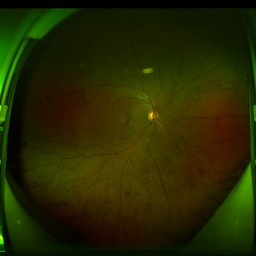
\includegraphics[width=0.42cm]{img/u1.jpg}};
  \draw[cU,line width=0.55pt] (th.south west) rectangle (th.north east);
  \draw[cU,line width=0.4pt] (th.south) -- ([yshift=2.3pt]s);
  \draw[#2,line width=0.6pt] (0,0) rectangle (\pw,\ph);
\end{scope}}
\node[sml,anchor=north,inner sep=0pt] at (\qc,\hy) {inside the DR queue $\cdot$ ultra-widefield stream};
\node[ttl,anchor=north west,inner sep=0pt] at (\xa,\ty) {PROTON \textcolor{mute}{\mdseries$\cdot$ plain mean}};
\node[sml,anchor=north west,inner sep=0pt] at (\xa,\ny) {\shiftedPct\% shifted members pull the mean (\tikz[baseline=-0.6ex]{\draw[ink,line width=0.8pt,line cap=round] (-1.4pt,-1.4pt)--(1.4pt,1.4pt) (-1.4pt,1.4pt)--(1.4pt,-1.4pt);})};
\embedpanel{\xa}{line}{\pAx}{\pAy}{%
  \foreach \x/\y/\w in \memIDA \fill[cD,draw=white,line width=0.25pt] (\x,\y) circle (1.1pt);
  \foreach \x/\y/\w in \memUWFA \fill[cU,draw=white,line width=0.25pt] (\x,\y) circle (1.1pt);}{\pcross{p}{ink}}
\node[ttl,anchor=north west,inner sep=0pt,text=acc] at (\xb,\ty) {PROTON+ \textcolor{acc!75}{\mdseries$\cdot$ domain-anchored}};
\node[sml,anchor=north west,inner sep=0pt,text=acc] at (\xb,\ny) {\ding{172}\ shifted members get \weightPct\% of the weight};
\embedpanel{\xb}{acc}{\pBx}{\pBy}{%
  \foreach \x/\y/\w in \memIDB {\pgfmathsetmacro{\op}{0.45+0.55*\w}\fill[cD,fill opacity=\op,draw=white,line width=0.25pt] (\x,\y) circle (1.1pt);}
  \foreach \x/\y/\w in \memUWFB \draw[cU,fill=white,line width=0.45pt] (\x,\y) circle (1.05pt);}{\node[text=acc,font=\fontsize{12}{12}\selectfont] at (p) {$\star$};}
% verdicts (below the plots)
\node[verdict,fill=mute,anchor=north west] (v1) at (\xa,\vy) {missed};
\node[lbl,anchor=base west] at ($(v1.base east)+(0.08,0)$) {$S_{\mathrm{proto}}=\spA$};
\node[verdict,fill=cU!85!black,anchor=north west] (v2) at (\xb,\vy) {flagged as OOD};
\node[lbl,anchor=base west] at ($(v2.base east)+(0.08,0)$) {$S_{\mathrm{proto}}=\spB$};
% legend (centred under the block)
\node[sml,anchor=north,inner sep=0pt] at (\qc,\cyb-0.10) {%
  \tikz[baseline=-0.6ex]\fill[cN] circle (1.25pt);\ normal\hspace{5pt}%
  \tikz[baseline=-0.6ex]\fill[cD] circle (1.25pt);\ DR\hspace{5pt}%
  \tikz[baseline=-0.6ex]\fill[cU] circle (1.25pt);\ ultra-widefield (shifted)\hspace{5pt}%
  \tikz[baseline=-0.6ex]\draw[cU,fill=white,line width=0.45pt] circle (1.15pt);\ ${\approx}0$ weight\hspace{5pt}%
  \tikz[baseline=-0.6ex]\draw[ink,line width=0.8pt] circle (1.9pt);\ real image, softmax \conf\ ``DR''};
\end{tikzpicture}
\end{document}
